\begin{figure}[p]\centering
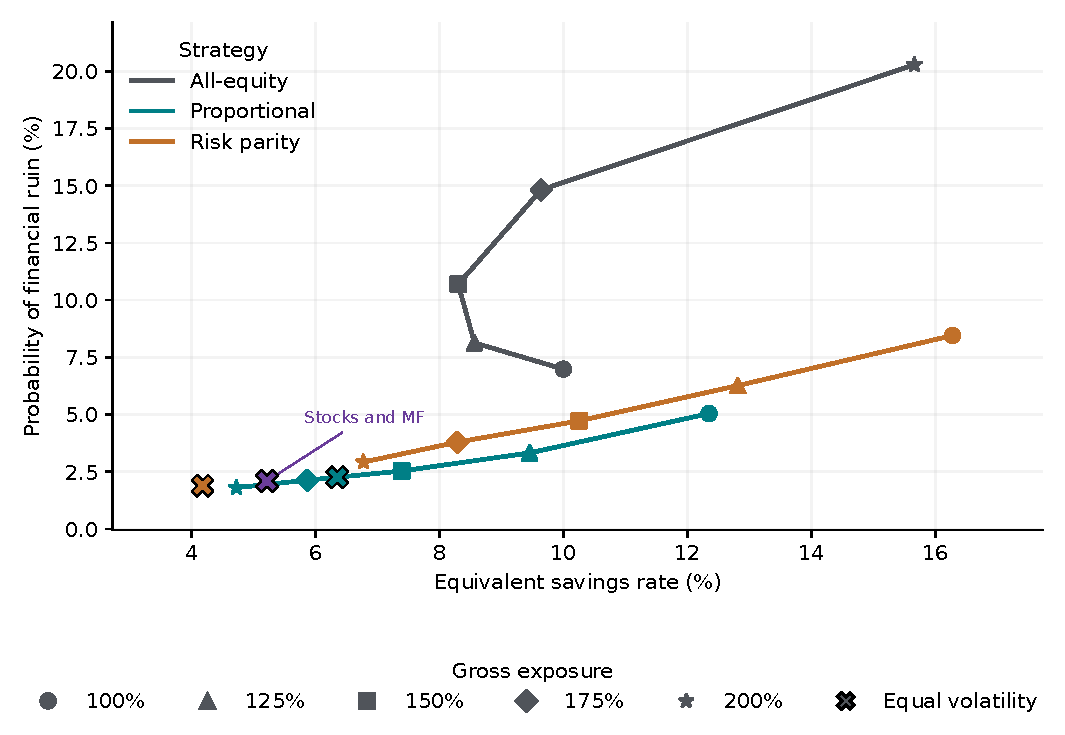
\includegraphics[width=\linewidth]{figures/erc/ladders.pdf}
\caption{Equivalent savings rates and ruin probabilities. The figure plots the probability of financial
ruin against the equivalent savings rate for the all-equity, proportional, and risk parity strategies at
gross exposures of 100\%, 125\%, 150\%, 175\%, and 200\%. Crosses mark the proportional, risk parity, and
stocks-and-managed-futures strategies at the volatility of the unlevered all-equity strategy (166\%, 265\%,
and 132\% exposure). The equivalent savings rate equates expected utility with that of the all-equity
strategy at 100\% exposure and a 10\% savings rate. Results are based on 10,000 bootstrap simulations from
the 1927 to 2025 sample.}
\label{fig:ladders}
\end{figure}
